\documentclass[10pt, conference, compsocconf]{IEEEtran}

\title{Mitigating DDoS attacks in Named Data Networking}%:\\ Cache/Content Poisoning}
\author{anonymous}

\usepackage{graphicx}
% \usepackage[colorlinks]{hyperref}
\usepackage[]{hyperref}
\usepackage{breakurl}
\usepackage{url}
\usepackage[nocompress]{cite}
% \usepackage{verbatim}
% \usepackage{algpseudocode}
\usepackage{algorithm}
\usepackage{algpseudocode}

\newcommand{\note}[1]{\vspace{2 mm}\par \noindent \textsc{Note}
\framebox{\begin{minipage}[c]{0.40 \textwidth}
\tt #1 \end{minipage}}\vspace{5 mm}\par}

\newcommand{\todo}[1]{\vspace{2 mm}\par \noindent \textsc{ToDo}
\framebox{\begin{minipage}[c]{0.42 \textwidth}
\tt #1 \end{minipage}}\vspace{5 mm}\par}

\begin{document}
\maketitle

\begin{abstract}

Distributed Denial of Service attack is an ongoing problem in today's Internet. 
A newly proposed future Internet architecture, Named Data Networking (NDN), lets end users request desired data by sending Interest packets, and the network forwards data packets to end users upon request only. 
Thus, NDN can effectively defeat the existing DDoS attacks, however it can be subject to new types of DoS attacks, namely Interest packet flooding.  
In this paper we investigate effective solutions to mitigate Interest flooding attacks. 
We use simulations to evaluate the design and our results show that our proposed solution can respond to Interest flooding attacks quickly, and that the inherent flow-balance property of NDN (i.e., one Interest packet retrieves at most one Data packet) can be used as a basis for effective DDoS mitigation algorithms.

\end{abstract}

\begin{IEEEkeywords}
Information-Centric Networks, Named-data Networking, Denial-of-Service
\end{IEEEkeywords}

\section{Introduction \label{intro}}
Denial of service (DoS) and distributed denial of service attacks (DDoS) appeared not very long time after Internet got traction and since then a constant arms race is going on between information providers and attackers who want to knock a certain source of information down. Running a DDoS attack has become a very successful business model due to its general scalable nature, cheapness and lack of protection of information providers by government and law. Most popular and economically effective DDoS attacks are organized with botnets. A botnet agents get installed by many various ways on computers of ordinary people that leads to a very wide geographical distribution of the source of attack that makes blacklisting impossible (in contrast to single source DoS attacks).

In 2011 for the first time IPv6 DDoS attacks on commercial networks were observed. They occur rarely, but it only means that IPv6 is not widespread enough for attackers to put significant resources into such DDoS attacks. Principally, in terms of DDoS security IPv6 didn't advance that much comparing to standard IPv4 networks.

IP architecture has a wide surface for denial of service attacks which takes the beginning from the thin-waist IP protocol, goes through transport level and up to DNS level. In IP it is very easy to forge source address and specify the exact destination that needs to be placed under attack that creates possibilities to perform various types of reflection DoS attacks. On transport level in TCP/IP SYN flood, RST flood and FIN-way attacks are very effective and popular. DNS system can be attacked in multiple ways, e.g. DNS amplification attack. 

We believe that future Internet architectures can do and must do more for DDoS prevention. By its design NDN architecture is not sensitive to any kind of reflection attacks due to the lack of host addresses and ubiquitous data caching. NDN architecture can operate without any DNS-like architecture since it routes and forwards packets based on human-readable names instead of IP addresses that need to be resolved with DNS. 
  
%\todo{
%Current Internet architecture and its resilience to DoS and DDOS. Requirements from a new architecture such as CCN with respect to DoS and DDoS resilience.

%Our contributions.

%Paper organization.}

In this paper we provide a brief overview of possible DDoS attacks in NDN architecture, analyze all aspects of Interest flooding attack in NDN architecture, propose multiple defensive techniques against such attacks, establish evaluation methodology using ndnSIM simulation software, execute small scale and Internet scale attack scenarios, and analyze our experimental results.

Following this introduction, Section 2 gives a brief overview of NDN architecture, and Section 3 lists and overviews possible attack in NDN. Section 4 thoroughly discusses Interest flooding attack, and Section 5 proposes multiple defensive techniques against it. Section 6 describes evaluation methodology and gives experimental results. Section 7 provides analysis based on our results. Section 8 concludes and describes future work.

%\begin{figure}[htpb]
%  \centering
%  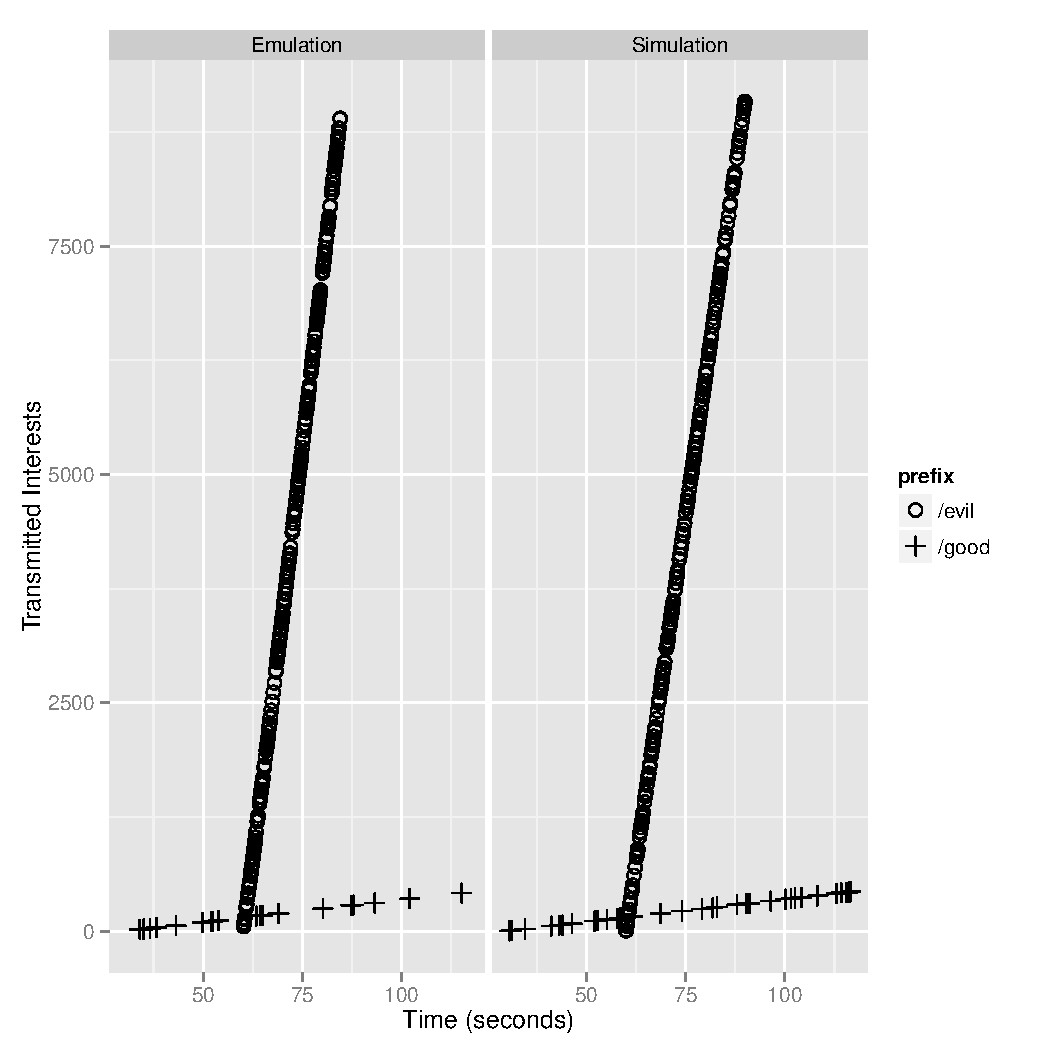
\includegraphics[scale=0.5]{figures/sim-emu-power.pdf}
%  \caption{Strength of Interest flooding attack}
%  \label{fig:simemupower}
%\end{figure}

%\begin{figure}[htpb]
%  \centering
%  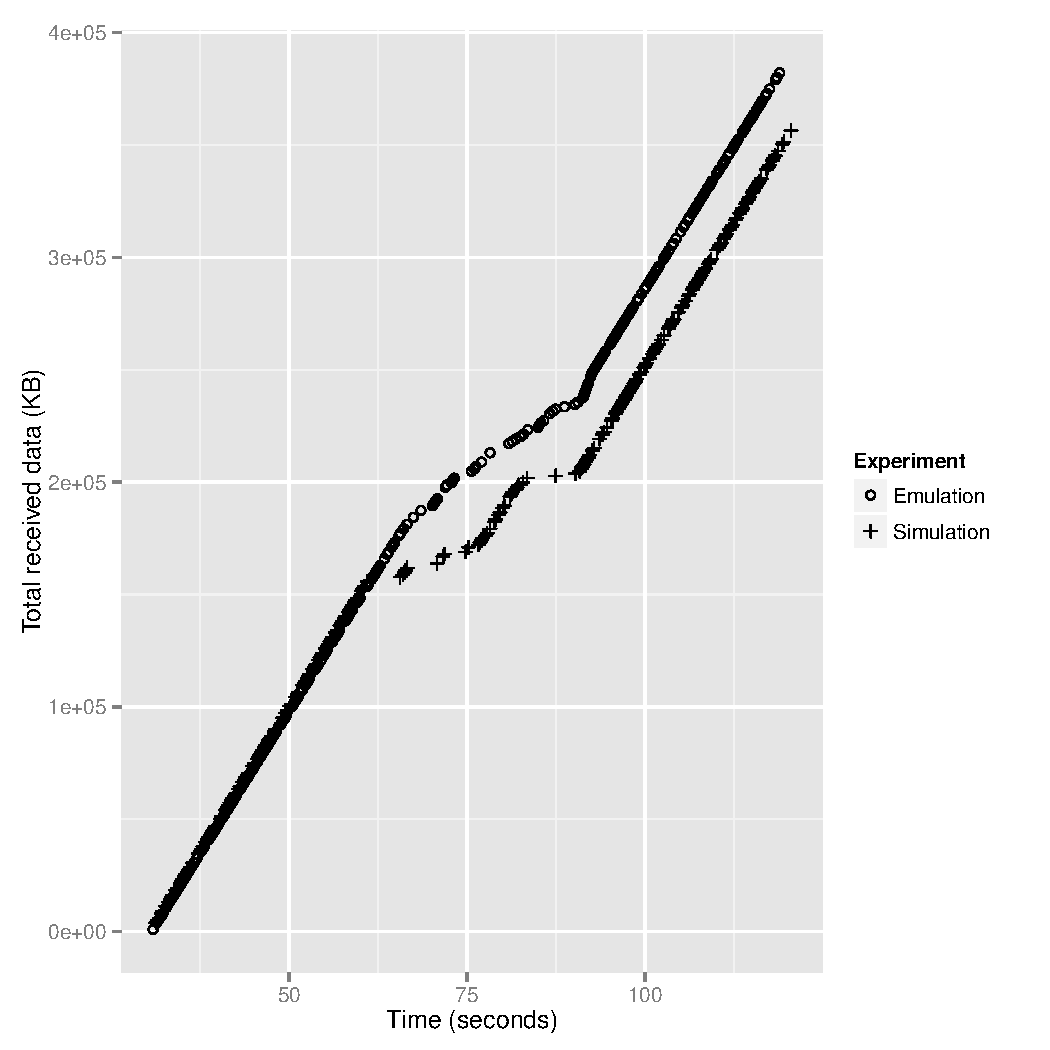
\includegraphics[scale=0.5]{figures/sim-emu-performance.pdf}
%  \caption{Data retrieval by legitimate clients}
%  \label{fig:simemuperf}
%\end{figure}


\section{ NDN Overview\label{ccn-intro}}
Named Data Networking (NDN) is a network architecture which aims to replace IP architecture by replacing IP�s host-to-host data delivery model with pull-based information retrieval model. In IP in order to retrieve data, data consumer have to know endpoint location of the desired data, in NDN all they have to know is data name. Names are hierarchical (non-flat) application-defined string names that are used for forwarding, routing and caching. A canonical NDN name looks in a following way: /ndn/ucla/CSdept/faculty/Lixia/webpage.

NDN communication uses two packet types: Interest and Data. An Interest packet contains data name and is issued by the receiver to express what data is needed. The sender puts a data packet into the network in response to an Interest. An Interest is �satisfied� when a Data packet is received with matching data name.

Every NDN node manages three important data structures:
\begin{enumerate}
\item{Forwarding Interest Base (FIB) maps name prefixes and multiple physical network interfaces (where to forward Interests). Having one-to-many relationship in this table allows multipath forwarding of Interests.}
\item{Content Store (CS) temporarily stores Data packets that pass through this node and allows fast Data retrieval.}
\item{Pending Interest Table (PIT) holds all "not yet satisfied" Interests that have been sent upstream. Every element contains a list of incoming and outgoing physical interfaces to enable multipath Interest forwarding and multipath Data delivery.}
\end{enumerate}

So how it works altogether? Every incoming Interest triggers a lookup in the Content Store and if the Data with matching data name have been found, it is sent back to the same physical interface from which the Interest has arrived. If CS lookup is unsuccessful, Interest must be sent further upstream and put in the PIT. However, all recurring Interests with the same prefix name are stacked together in the same PIT entry and are not sent to the upstream again until this PIT entry expires completely because of timeout. If Data returns from some upstream location it is replicated for each incoming physical interface stored in this PIT entry after that it is removed from PIT. In other words, multipath Data delivery is built-in in NDN. 


%\begin{figure}[htpb]
%  \centering
%  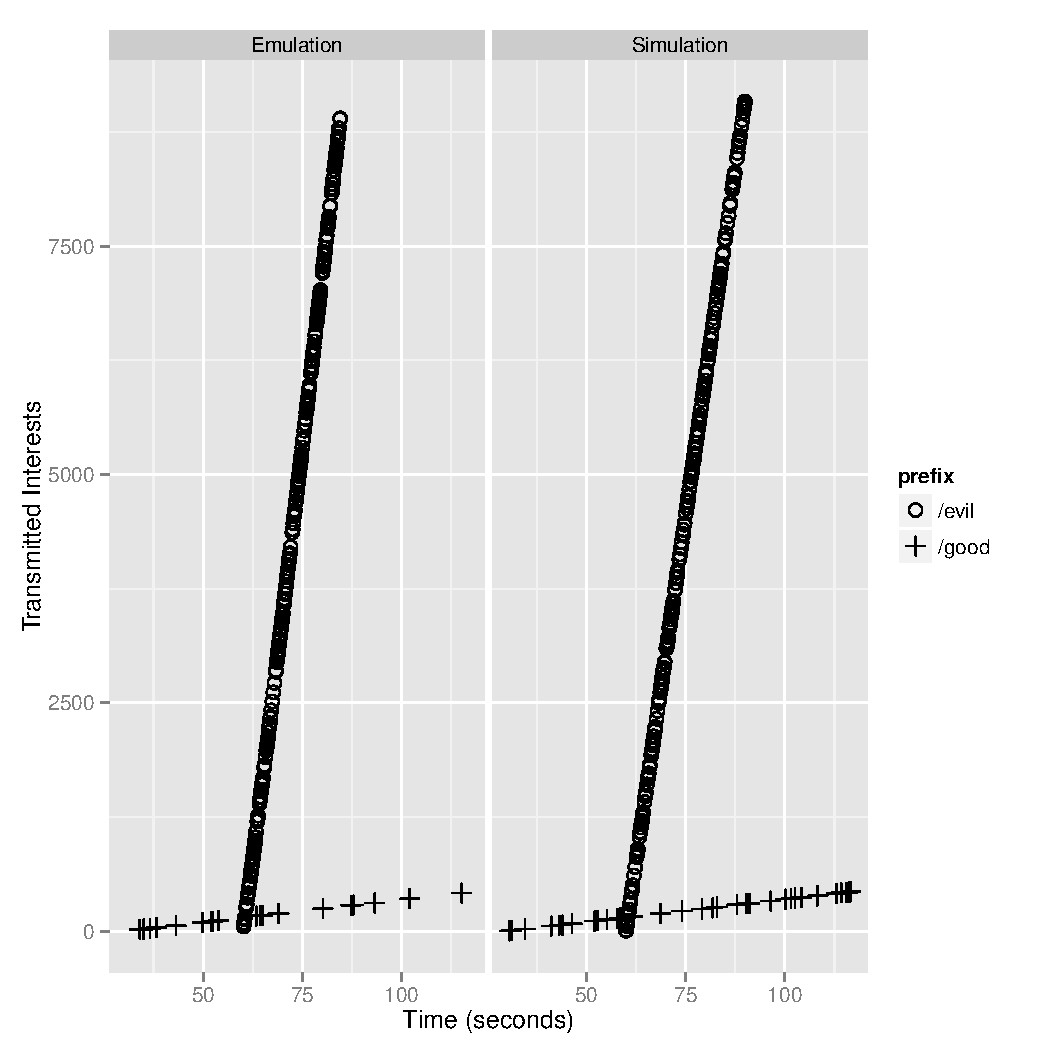
\includegraphics[scale=0.5]{figures/sim-emu-power.pdf}
%  \caption{Strength of Interest flooding attack}
%  \label{fig:simemupower}
%\end{figure}

%\begin{figure}[htpb]
%  \centering
%  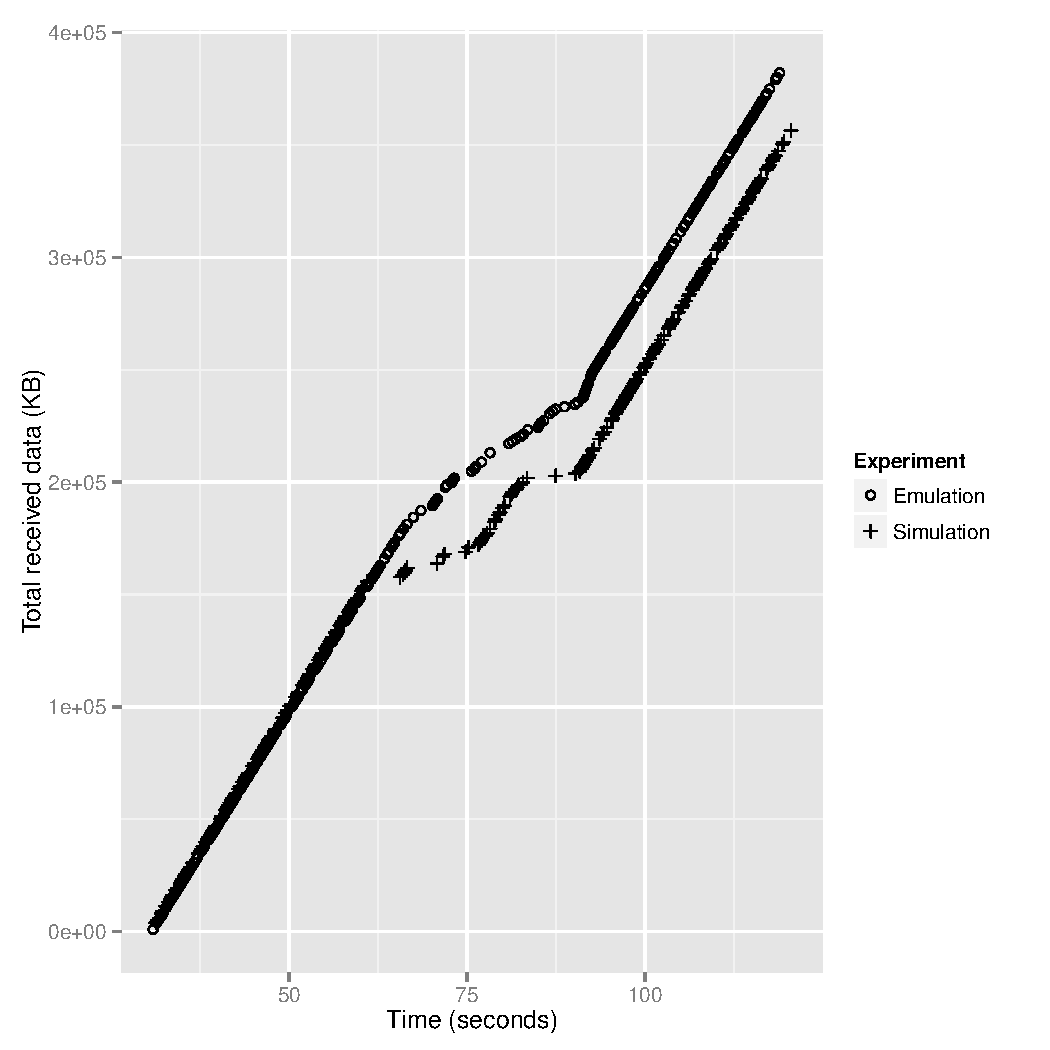
\includegraphics[scale=0.5]{figures/sim-emu-performance.pdf}
%  \caption{Data retrieval by legitimate clients}
%  \label{fig:simemuperf}
%\end{figure}


\section { DDoS Attacks in NDN \label{ddos-ndn}}
Brief overview of possible attacks in NDN, and scope of what we will tackle in this paper (Interest flooding).



  
%\begin{figure}[htpb]
%  \centering
%  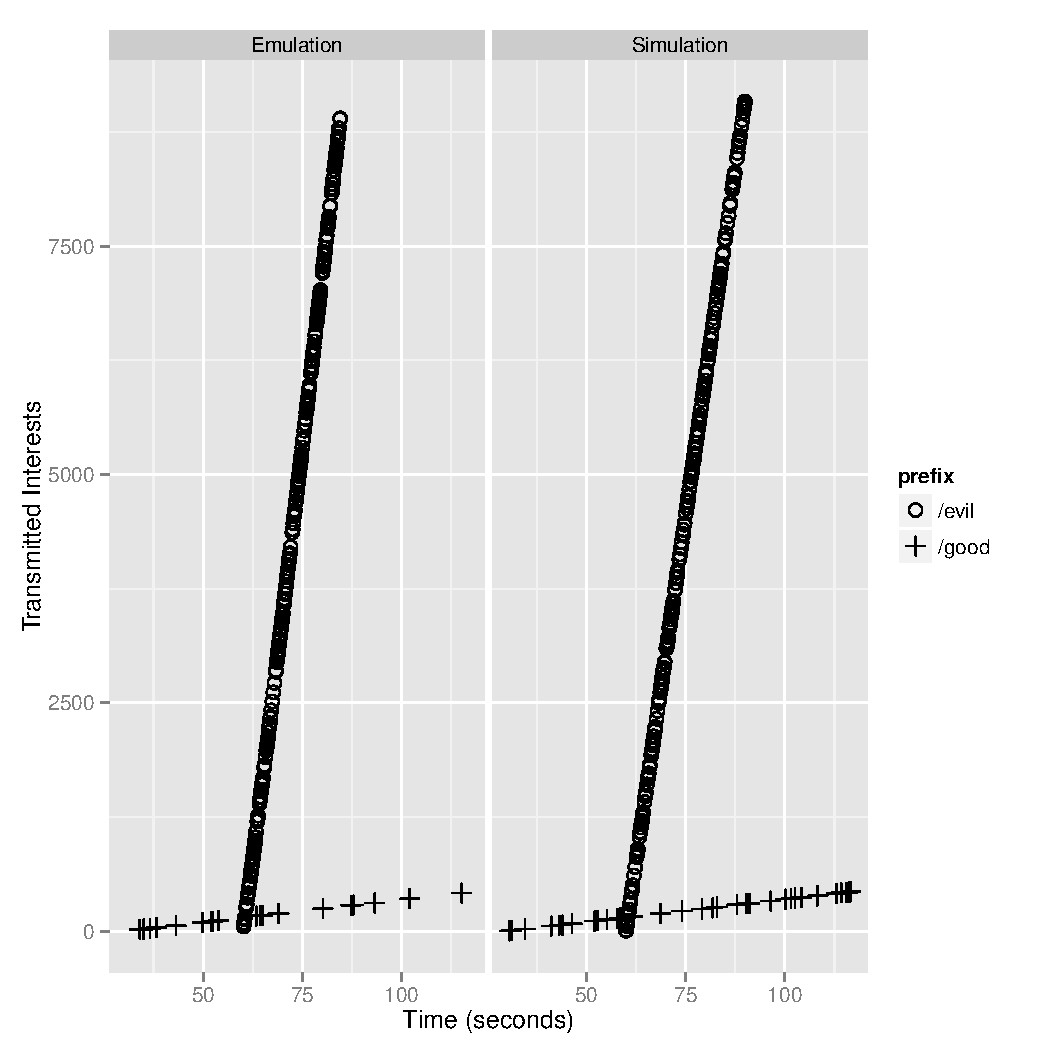
\includegraphics[scale=0.5]{figures/sim-emu-power.pdf}
%  \caption{Strength of Interest flooding attack}
%  \label{fig:simemupower}
%\end{figure}

%\begin{figure}[htpb]
%  \centering
%  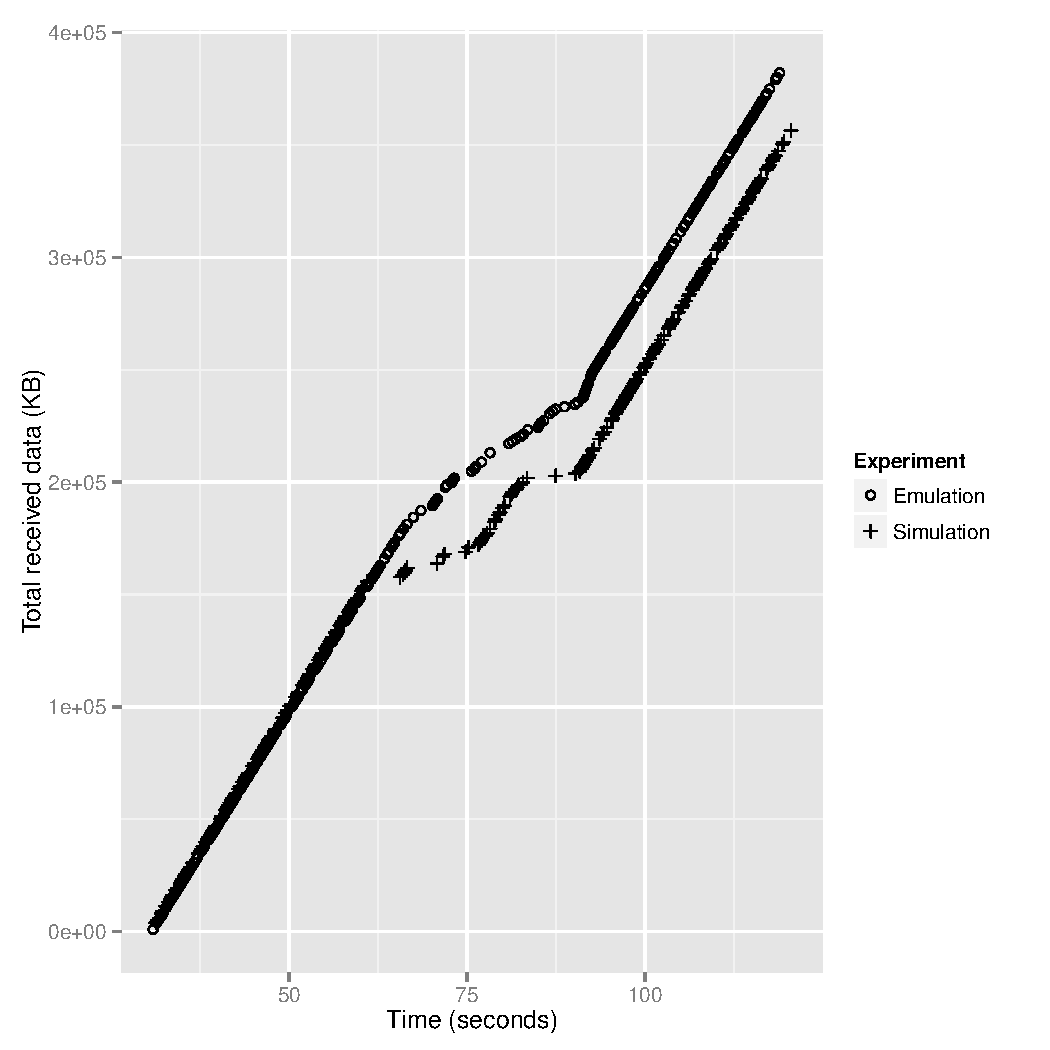
\includegraphics[scale=0.5]{figures/sim-emu-performance.pdf}
%  \caption{Data retrieval by legitimate clients}
%  \label{fig:simemuperf}
%\end{figure}


\section { Interest Flooding in CCN }

\section {Countermeasures against Interest flooding}

Basic limits, probablity based on statistics, and dynamic window adjustment

(Description of each of the above, and their implications) 

\section {Evaluation}
\todo{Both simulation, as well as emulation for various sized topologies (trees as well as real topologies), various parameters etc.
List all possible parameters, say clearly which ones we vary, and which ones we do not, along with explanations.

Metrics that we will consider in our evaluation (Satisfaction rate for good clients, Link utilization near producers, Latency for good clients, good versus bad interests as a function of time).}

We want to explore the effectiveness of designed mitigation techniques in a two distinctive ways. First, we need to understand how each method works on a very ground level of a just few nodes and links. Second, we want to pick promising techniques and see if they work in a large scale networks of hundreds and thousands of nodes. To ensure the correct transition from small scale experiments to large scale experiments we had to use the same evaluation tool in order to eliminate any possibility of implementation discrepancy. As of today the only network simulator supporting full NDN logic is the NS-3 based ndnSIM software. 

\subsection{Simulation versus Emulation}
\label{sec:simemu}
Before committing significant efforts into simulation-based implementation of designed defensive techniques it was necessary to confirm that ndnSIM has close performance characteristics to the reference NDN implementation - Project CCNx. This will guarantee that evaluation results derived from simulations will be meaningful in real NDN world.

To achieve this goal a comparison of Project CCNx software and ndnSIM software was performed under small scale Interest flooding attack. DETER Testbed was used as emulation tool for CCNx evaluation. Using it we were able to setup non-virtualized Ubuntu nodes running CCNx 0.6.0 software connected in a binary tree topology with 4 leaves and 1 root node. A number of applications running on top of CCNx have been developed, namely:
\begin{itemize}
\item{Producer application serves 1KB data packets under a known for the attacker name prefix}
\item{Legitimate client application requests 5KB of data per second from the producer}
\item{Attacker application tries to fill the channel of the producer by sending 500 Interest packets per second}
\end{itemize} 

In this emulation scenario producer application occupied a root node, legitimate clients occupied all even leaves and attacker applications were put on all odd leaves. With 100kb links with 40ms delay such setup leads to no congestion during the period when attackers are turned off and congestion when they are turned on (seconds 60-90). Exactly the same scenario was replicated for ndnSIM evaluation, however, we had to adjust the sending rate of attacker application in order to produce the same amount of congestion in the network. Sending rates are compared in Figure~\ref{fig:simemupower}. To achieve the identical slope and height of sending rate of evil Interests by attacker nodes we had to reduce sending rate of simulation-based attacker application by 30\%. The most likely reason for that is the overhead of Java virtual machine and operating system itself during the emulation of CCNx that results in eventual 30\% slower Interest transmission.  

Once we achieved the same characteristics of Interest flooding attack we were able to compare data packet losses by legitimate clients. Figure~\ref{fig:simemuperf} shows the cumulative received data by legitimate consumers in emulation and simulation experiments. NdnSIM performs worse due to its more deterministic nature, while the effects of UDP protocol usage, operating system process scheduling, and other kernel level operations on packet queues provide more randomness and a better intermixing of bad and good traffic which gives a slightly better performance. To summarize, we can use ndnSIM for our evaluations and real world performance is likely to be even better than our evaluation results.

\begin{figure}[htpb]
  \centering
  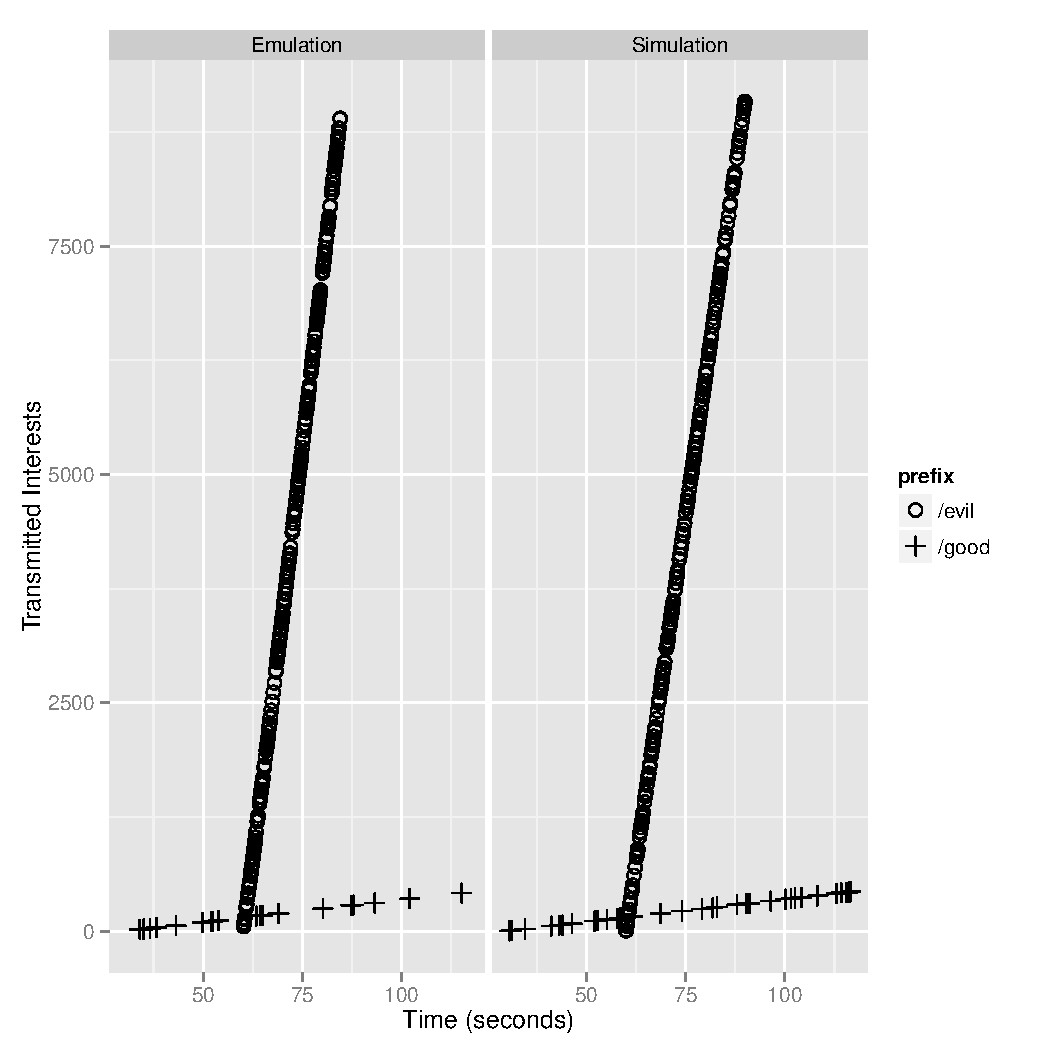
\includegraphics[scale=0.5]{figures/sim-emu-power.pdf}
  \caption{Strength of Interest flooding attack}
  \label{fig:simemupower}
\end{figure}

\begin{figure}[htpb]
  \centering
  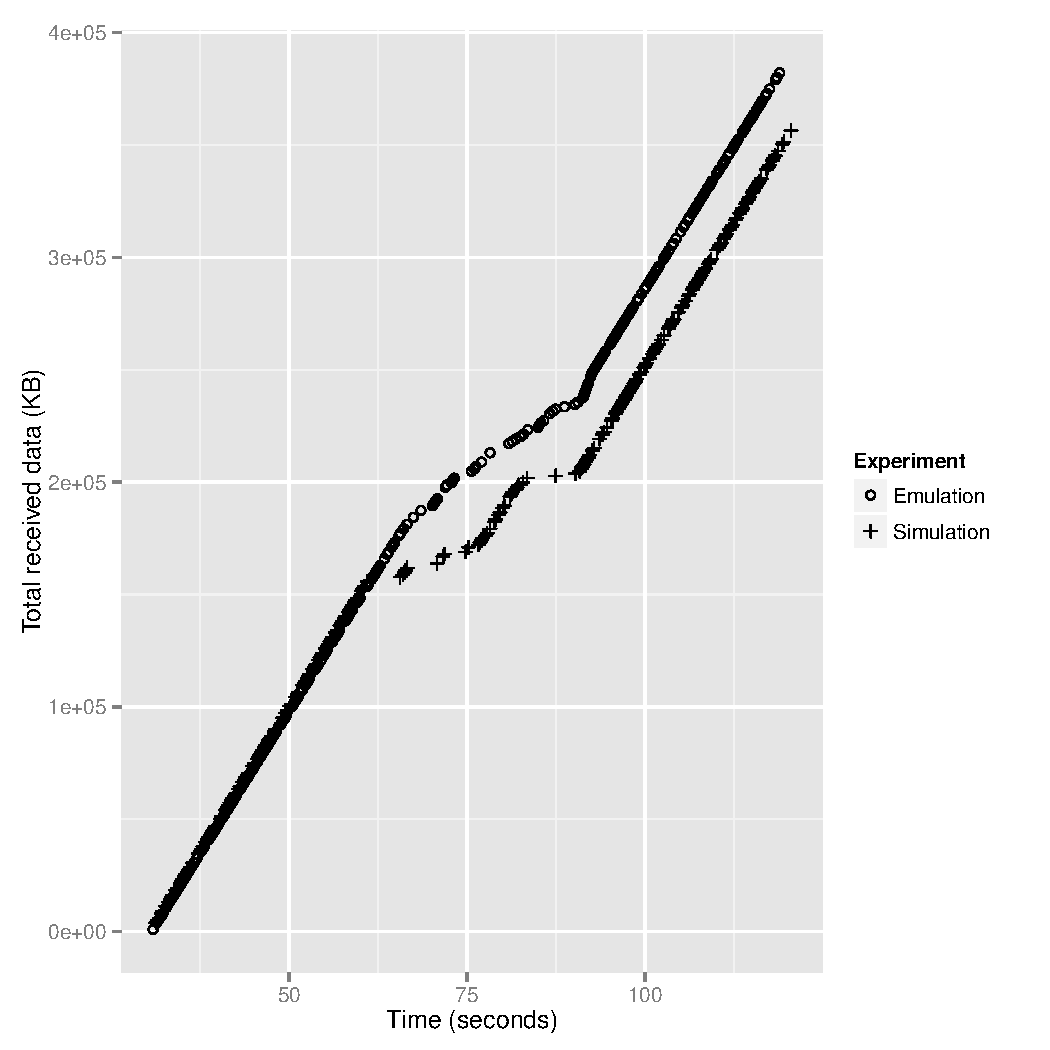
\includegraphics[scale=0.5]{figures/sim-emu-performance.pdf}
  \caption{Data retrieval by legitimate clients}
  \label{fig:simemuperf}
\end{figure}




\subsection{Results from probability based on statistics}

\subsection{Results from dynamic window adjustment}

\subsection{Large scale simulations}
\label{sec:largescale}

Large scale, large scale

%\begin{figure}[htpb]
%  \centering
%  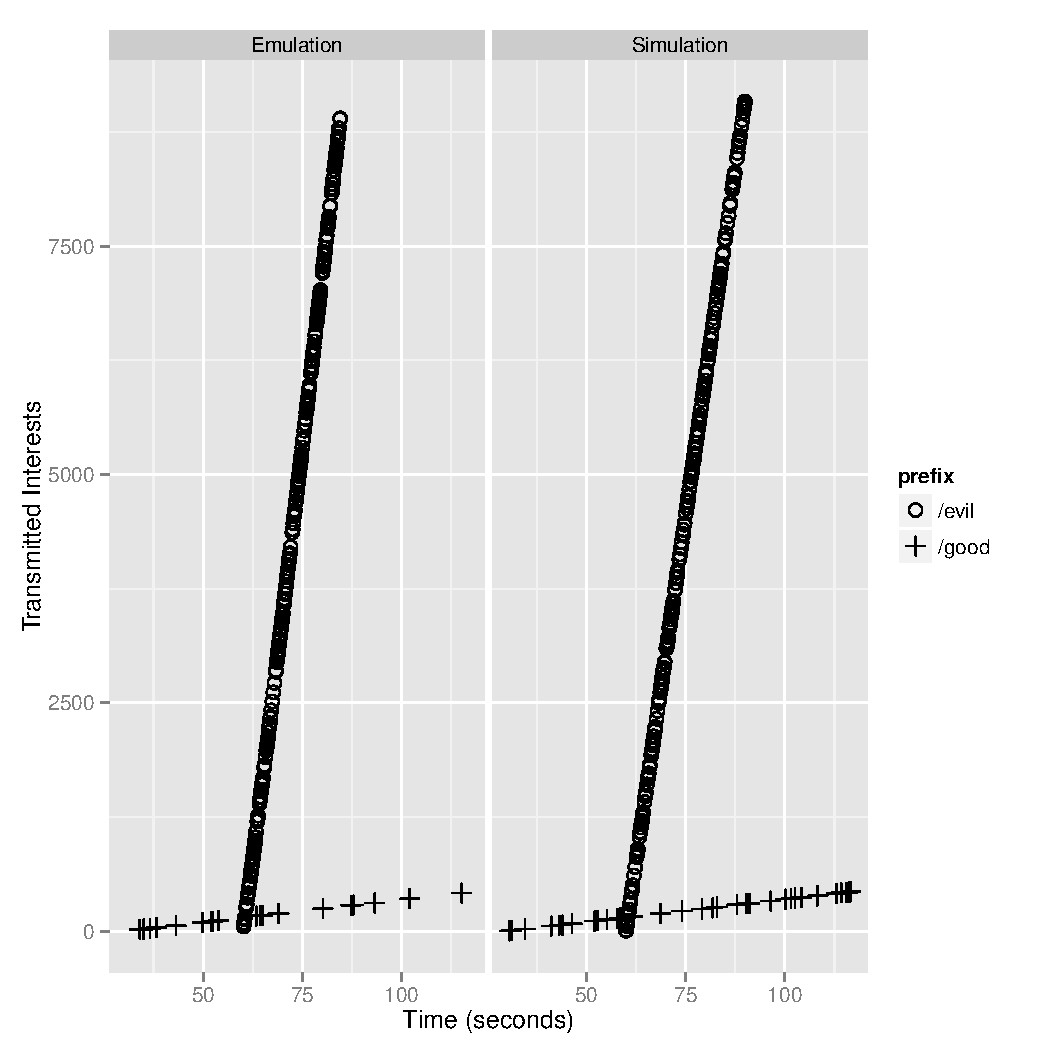
\includegraphics[scale=0.5]{figures/sim-emu-power.pdf}
%  \caption{Strength of Interest flooding attack}
%  \label{fig:simemupower}
%\end{figure}

%\begin{figure}[htpb]
%  \centering
%  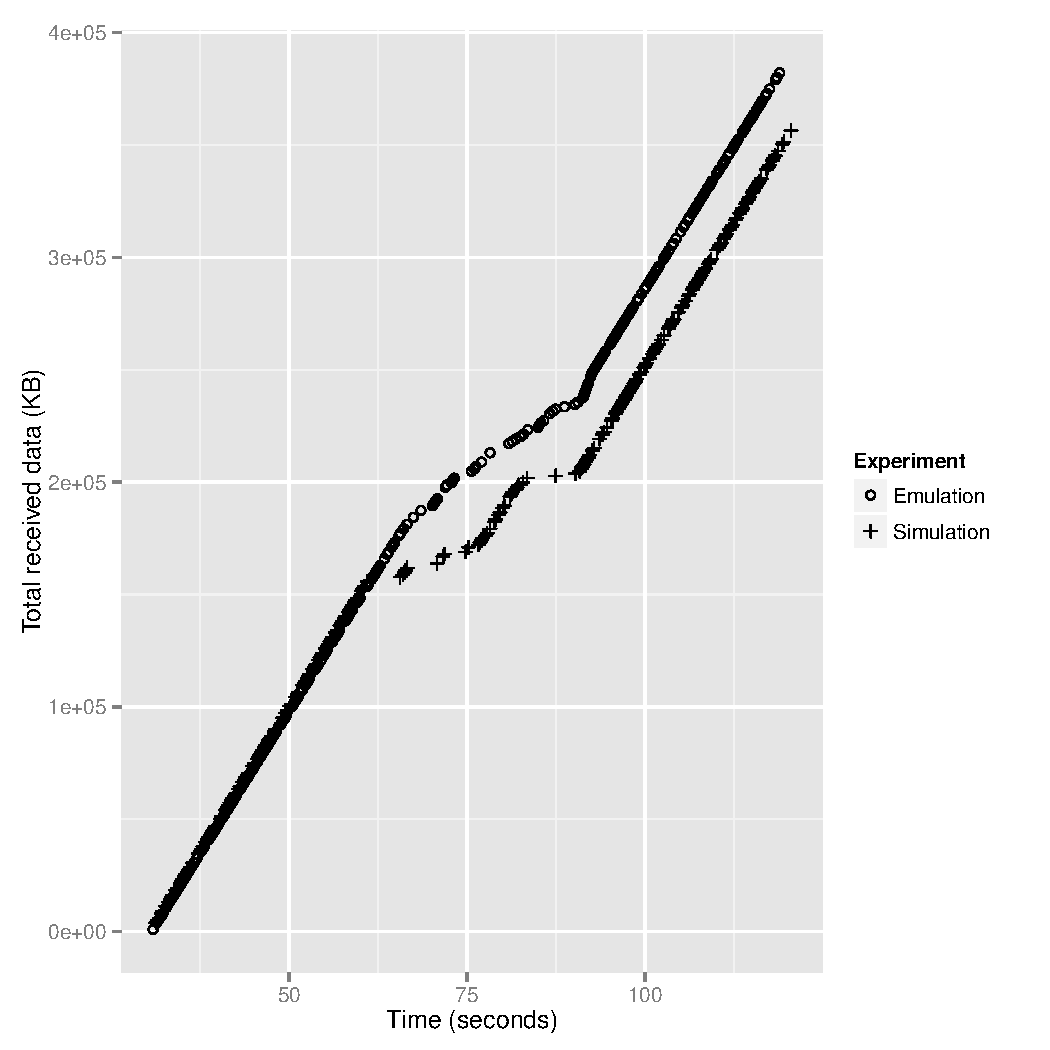
\includegraphics[scale=0.5]{figures/sim-emu-performance.pdf}
%  \caption{Data retrieval by legitimate clients}
%  \label{fig:simemuperf}
%\end{figure}



\section{Implications/Analysis}
Lessons we learnt, comparison of different mitigation techniques. 
Adapting these to mitigate other DDoS attacks.

\section{Conclusions and Future Work}

\bibliographystyle{plain}
\bibliography{references}

\appendix

\subsection{Physical limits}
\label{sec:physical limits}

The requirement to send an Interest in order to receive Data packet, provides an NDN consumer a unique opportunity to request the right amount of Data.
Moreover, the same opportunity to control the amount of data flow is given not only to consumers, but all routers between consumer and producer (or nearby caches).  
In other words, every node, either a consumer or an intermediate router, is able to control how much data it wants to receive by limiting the number of forwarded Interests.

The limitation can implemented in a number of different ways, including leaky bucket scheduling and window-based flow control.
We decided to following TCP-like window-based flow control and applied the sliding window approach to implement Interest limits.

The size of the window defines how many Interests can be send out before Interests get satisfied or expired.
From the one hand, this size should be large enough to ``fill the pipe,'' meaning that a node needs to send enough Interests to receive Data at full capacity of the incoming link.
On the other hand, the window's size should not be too large to avoid excessive buffering and congestion of the Data packet.
Thus, the ideal size for such a window need to be defined proportional to link's bandwidth-delay product~\cite{tcp-survey}.
With the objective to request as many Data packets, as downstream link can pump through, we are getting the following equation for Interest limit:

\[
\mathrm{Interest\ Limit} = Delay\ [s] \cdot \frac{\mathrm{Bandwidth\ [Bytes/s]}}{\mathrm{Data\ packet\ size\ [Bytes]}}
\]

Note that the value of \textit{Delay} is not known a priory and varies between different Interest-Data flows.
However, we do not need to know the exact value of the delay and can set it as an average round trip delay among all flows (with a reasonable filtering of outliers).
This way, the statistical traffic multiplexing with link-level buffering will allow full utilization of the downstream link.
Exactly the same reasoning can be applied to the \textit{Data packet size} parameter, which can also be set to an average observed Data packet size.

Unlike rate-based approaches, window-based limiting does not require precise knowledge about the rate, as well does not need precise scheduling mechanisms.
Like in TCP, the window-based flow is self-clocking, easily adjusting itself to any traffic patterns.

%%% Local Variables: 
%%% mode: latex
%%% TeX-master: "../paper"
%%% End: 


% \subsection{Physical limits with ``fair'' queuing}
% \label{sec:queuing}

% However, this limitation approach does not attempt to utilize data plane performance knowledge (i.e., Interest satisfaction ratio statistics) to discriminate good and malicious Interests.

To partially overcome deficiencies of the Physical limits algorithm we need to ensure that the forwarded Interests represent at least a ``fair'' mix of the Interests received from different neighbors (interfaces).
That is, if the routers A on Fig.~\ref{fig:flooding example} has a very tight token budget, these tokens should be fairly distributed between incoming interfaces \texttt{eth0} and \texttt{eth1}.
Because of the very small volume of Interests, we cannot simply rely on network buffers to do statistical multiplexing of Interests, as they would almost never be buffered.
At the same time, until bag of tokens is not empty, there is no reason to delay Interest forwarding, as we do not known how many and from which interfaces Interests will arrive in the future.
Therefore, in order to achieve the goal of ``fair'' mixing of Interests, we need to implement additional mechanisms to buffer and mix incoming Interests, only if they cannot be immediately forwarded.

For the buffering part, we can reuse Pending Interest Table, with a small extension to support flagging of the Interests that cannot be forwarded immediately (see example on Fig.~\ref{fig:queueing}). 
As for the mixing part, we need an additional fair queuing mechanism, which can be implemented in a form of hierarchical queues (on Fig.~\ref{fig:queueing})\footnote{This essentially is a class based queuing, with classes for each outgoing/incoming interface.} or using virtual time approach~\cite{zhang1990virtual}. 
It should be noted that unlike normal queuing, Interest queues do not actually store a packet, but merely a bi-directional pointer to the existing PIT entry.
This way, PIT entry can be quickly updated when the Interest is actually forwarded, as well as the element can be removed from the queue when the Interest expires.

\begin{figure}[htbp]
  \centering
  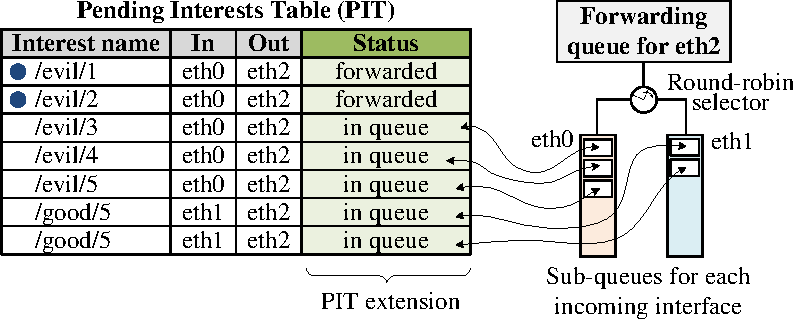
\includegraphics[scale=0.65]{queue}
  \caption{Interest queuing: if tokens are unavailable, the router creates PIT entry, but instead of forwarding, enqueued the Interest}
  \label{fig:queueing}
\end{figure}

A more formalized description of the Physical limits algorithms with per-interface fairness is presented in Pseudocode~\ref{alg:queuing}.
The algorithm extends the base Physical limits algorithm by enabling queuing when the bag of tokens is empty (lines 7--10), as well as by triggering an action (lines 16--21), when a token becomes available and enqueued Interest can be finally forwarded.
At the same time, the algorithm limits number of Interests allowed in a queue, constraining memory usage increase by at most a constant factor, compared to the base Physical limits algorithm (i.e., memory attack on routers are still unfeasible).


\floatname{algorithm}{Pseudocode}

%%%%%%%%%%%%%%%%%%%%%%%%%%%%%%
%%%%%%%%%%%%%%%%%%%%%%%%%%%%%%
%%%%%%%%%%%%%%%%%%%%%%%%%%%%%%

\begin{algorithm}[h]
\caption{Physical limits with per-interface fairness}
\label{alg:queuing}
\begin{algorithmic}[1]
\State{} \Comment{Same initialization, InData and Timeout functions as in Physical Limits algorithm}

\vspace{0.2cm}

\Function{OutInterest}{Interest \textbf{i}, InInterface \textbf{if}, OutInterface \textbf{of}}
    \If{$L_{of} - O_{of} > 0$} \Comment{\textbf{of} is under physical limits}
        \State $O_{of} \leftarrow O_{of} + 1$  \Comment{``Borrow'' token}
        \State add \textbf{of} to PIT entry and forward \textbf{i} to \textbf{of}
    \Else
        \State Queue $q \leftarrow of$.GetSubQueue($if$)
        \If{$Size(q) < L_{of}$}
           \State $q$.PushInterest($i$)
           \State add \textbf{of} to PIT entry, and link PIT entry with the queue
        \Else
           \State drop Interest
        \EndIf
    \EndIf
\EndFunction

\vspace{0.2cm}
\State{} \Comment{\textit{Whenever $L_{of} - O_{of}$ becomes larger than zero}}
\Function{TokenBecomesAvailable}{}
    \State Queue $q \leftarrow$ $of$.GetRoundRobinSubQueue 
    \State $i \leftarrow$ $q$.PopInterest
    \State update PIT entry and Forward($i$, $of$)
\EndFunction
\end{algorithmic}
\end{algorithm}


It should be noted that enqueued Interests should not be kept in the queue for a prolonged period of time.
Otherwise, by the time the Interests reaches the Data, the state could have been long expired downstream, effectively making such an Interest useless.
Additional mechanisms of pair-wise agreements between NDN routers and periodic Interest refresh can solve this particular problem, but it is out of the scope of the present paper.

As we show in Section~\ref{sec:evaluation}, fair queueing provides a partial relief from the Interest flooding attack, allowing legitimate users to successfully fetch Data for 15--20\% of the expressed Interests (compared to 0-10\% without fair queueing).
At the same time, the Physical limits with or without fair queueing allows attackers to send a relatively small volume of Interests in order to significantly impact service for the legitimate users.
Therefore, to successfully solve the problem, we need a more intelligent approach, allowing us to localize the attack traffic as close to the attack origin as possible.

%%% Local Variables: 
%%% mode: latex
%%% TeX-master: "../paper"
%%% End: 



% Differential treatment of Interests received from different interfaces can be achieved in a more elegant way, without reverting to probabilistic methods.

Essentially, the probabilistic Interest accept algorithm divides the available forwarding tokens between interfaces proportionally to their satisfaction ratios.
Exactly the same effect can be achieved without using probabilistic methods, simply by enabling and enforcing additional Interest limits for each incoming interface, where the values of the limits directly depend on the interface satisfaction ratios.
Additionally, routers may need to explicitly announce these limits to their downstream neighbors, ensuring that any forwarded Interest from the downstream is actually getting through, resulting in genuine Interest satisfaction statistics.

The formal definition of the dynamic limits algorithm is presented in Pseudocode~\ref{alg:dynamic limits}, while Fig.~\ref{fig:dynamic limits example} illustrates how the algorithm would work in our toy example on Fig.~\ref{fig:flooding example}.
Assuming the initial (physical) limit $L=10$ and the current satisfaction ratios on the the router A are 50\% for \texttt{eth1} and 0\% for \texttt{eth0}, and on the router B the ratio is 30\%  \texttt{eth0}, each node would set and announce the following  incoming interface limits $L'$: 
\begin{enumerate}
\item the router B would set and announce the incoming interface limit $L'=3$;
\item the router A, after receiving announcement from B would readjust its incoming interface limits to $L'_{eth1} = 1.5$ and $L'_{eth0} = 0$; and
\item legitimate user and adversary may either obey or ignore the announced limit, which will be in any case enforced by the router A.
\end{enumerate}


\begin{figure}[htbp]
  \centering
  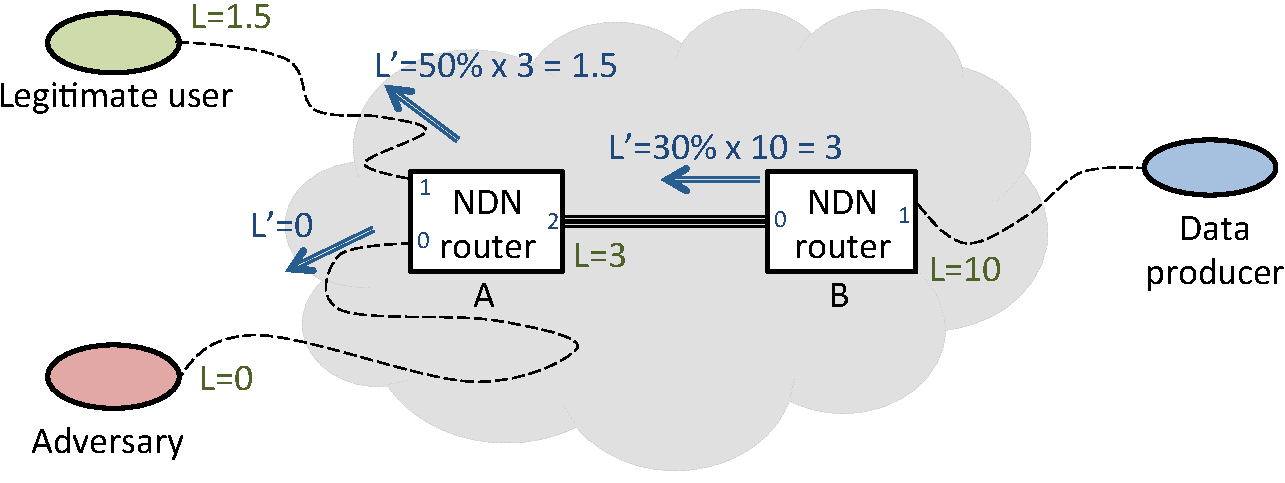
\includegraphics[width=\columnwidth]{dynamic-limits}
  \caption{Dynamic limits example: routers explicitly tell neighbors how many Interest can be for sure delivered to the Data producer}
  \label{fig:dynamic limits example}
\end{figure}


\floatname{algorithm}{Pseudocode}

%%%%%%%%%%%%%%%%%%%%%%%%%%%%%%
%%%%%%%%%%%%%%%%%%%%%%%%%%%%%%
%%%%%%%%%%%%%%%%%%%%%%%%%%%%%%

\begin{algorithm}[h]
\caption{Dynamic limits}
\label{alg:dynamic limits}
\begin{algorithmic}[1]
\State{} \Comment{Same initialization, InData and Timeout functions as in Physical Limits algorithm}
\vspace{0.2cm}
\State{$\forall f \in \mathrm{interfaces} : L'_{f} \leftarrow L_{f}$} \Comment{Per-incoming interface Interest limit} 

\vspace{0.2cm}

\State{} \Comment{\textit{Announcement from the neighbor}}
\Function{InLimits}{InInterface $if$, Limit $L'$}
    \State $L_{if} \leftarrow L'$
\EndFunction

\vspace{0.2cm}

\Function{AnnounceLimits}{} \Comment{\textit{E.g., every second}}
\For{\textbf{each} outgoing interface $of$}

   \For{\textbf{each} incoming interface $if$}
        \State $L'_{if}= {L_{of}} \times (1 - U_{if}/F_{if})$
        \State AnnounceLimit($if$, $L'_{if}$)
   \EndFor

\EndFor
\EndFunction

\end{algorithmic}
\end{algorithm}

The zero limit for the adversary's link means that the router A is temporarily not willing to accept any interests from this link, not until the statistics decays to the appropriate level (recall Fig.~\ref{fig:ratio example}).
At the next iterations of the dynamic limits algorithm, the legitimate user will be able to gradually improve the statistics on both the router A and router B (all his Interests will get through and will return Data), eventually resulting in a full allowance ($L'=L=10$) in the links between the routers A and B, and the user and the router A.

It should be noted that while in the description of the dynamic limits algorithm we used notions of ``outgoing'' and ``incoming'' interfaces, in the real system all interfaces can be both incoming and outgoing.
Thus, it may not be entirely clear which outgoing limit $L_{of}$ (line 10 in the algorithm) should be used to calculate the incoming limit $L_{if}$.
To overcome this problem, in our actual implementation we enforced separate incoming/outgoing interface limits for each individual FIB entry.
That is, for each FIB entry we set a separate Interest limit for each incoming interface ($L'_{{if}^{FIB}}$) based on a sum of FIB entry limits for each outgoing interface $L=\sum{L_{{of}^{FIB}}}$.


% Alex: not sure if this paragraph belongs here
Essentially, both probabilistic Interest accept and the dynamic limits algorithm are forms of a well-known push-back mechanism~\cite{Pushback}, with several core differences.
First, we are suppressing (pushing back) unwanted requests for Data, not the actual Data.
Second, differentiating between good and bad Interests is based on the traffic symmetry property of NDN.
% Alex: I'm not entirely sure about this point... 
Finally, both intelligent attack mitigation algorithms can be enabled all the time, without degrading network performance when there are no active attack.


%%% Local Variables: 
%%% mode: latex
%%% TeX-master: "../paper"
%%% End: 



Having successfully implemented a technique to gather statistics on Interest satisfaction ratios, our next challenge is in using this rotio to penalize malicious Interests. A straightforward method to achieve this enforcement is to use the Interest satisfaction ratio as a direct probability for accepting (forwarding) or rejecting an incoming Interest (see Pseudocode~\ref{alg:probabilistic model}).
%Apart from the Interest satisfaction statistics generation, there is a question how this statistics can be used to actually enforce prioritization and penalizing of Interests.


\floatname{algorithm}{Pseudocode}

%%%%%%%%%%%%%%%%%%%%%%%%%%%%%%
%%%%%%%%%%%%%%%%%%%%%%%%%%%%%%
%%%%%%%%%%%%%%%%%%%%%%%%%%%%%%

\begin{algorithm}[h]
\footnotesize
\caption{\small Satisfaction-based Interest acceptance}
\label{alg:probabilistic model}
\begin{algorithmic}[1]
\State{} \Comment{Same init, InData and Timeout functions as in Pseudocode~\ref{alg:queuing}}

\vspace{0.1cm}
\Function{OutInterest}{Interest \textbf{i}, InInterface \textbf{in}, OutInterface \textbf{out}}

    \State{} \Comment{Use uniform probability distribution model $P(X)$}
    \State{} \Comment{$P(X) : \forall x \in [0,1] \Rightarrow P(x) = x$}
    
    \If{$F_{in} > \theta $} \Comment{At least some Interests were forwarded before}
        \State $s \leftarrow (1 - U_{in} / F_{in})$
        \State Drop interest with probability $P(s)$
    \EndIf

    \State{forward the Interest, subjecting to token bucket limits}
\EndFunction

\end{algorithmic}
\end{algorithm}

Parameter $\theta$ on line 5 of the Pseudocode~\ref{alg:probabilistic model} ensures that the probabilistic model is not enforced when the volume of Interests arriving at a particular interface is small. This step is critical---while we want to drop Interests from attackers, we also want to provide an opportunity for legitimate users to regain their share of resources after temporary Data delivery failures due to  congestion.

A drawback of the satisfaction-based Interest acceptance method is that each router on the path makes an independent decision on whether to forward or drop the Interest. 
As a result of these independent decisions,  the probability of legitimate Interests being forwarded decreases rapidly as the number of hops between the content requester and producer grows; worsening the Interest satisfaction statistics and resulting in further drops.
In example on Fig.~\ref{fig:flooding example}, the router A observes 50\% satisfaction rate for \texttt{eth1} and 0\% rate for \texttt{eth0}. 
At the same time, router B observes a 30\% satisfaction rate for its \texttt{eth0} interface.
Next time a legitimate Interest arrives at router A, it has a 50\% chance of being forwarded further, and if forwarded, it has only a $50\% \times 30\% = 15\%$ probability of being forwarded further towards the Data producer. With each increasing hop in the network, the probability of being forwarded to the next hop decreases significantly. 
One way to prevent this overreaction and unfair penalization is to ensure that the decision taken at each router on whether to forward or drop the Interest is not independent of the decision taken at preceding routers. An explicit notification such as a gossip protocol between neighboring NDN routers that specifies the volume of Interests each router is willing to forward will likely address this issue. We leave the implementation and evaluation of a gossip protocol to future work.
%{\color{red}Alex: we should state that it is out of scope of the paper to evaluate this issue}

%%% Local Variables: 
%%% mode: latex
%%% TeX-master: "../paper"
%%% End: 



% Note that there is a condition (line 6 in Pseudocode~\ref{alg:probabilistic model}) to check if there is a valid statistics point.
% This condition is extremely important, because it first provides a basis to distinguish between known facts (i.e., good or bad satisfaction ratio for the incoming interface) and unknown facts (e.g., the first time an Interests arrives on the interfaces).
% Second, it gives an opportunity to recover from a bad history (history of unsatisfied Interests) after malicious Interests are ceased to flow in.
% Essentially, this recovery relies on statistics module to perform time-based invalidation of historical data (timely, but not too quickly\footnote{Otherwise, attackers may send short bursts of malicious Interests, successfully avoiding differential Interest treatment}).


Pseudocode~\ref{algo:interest stats} formally defines per-incoming interface statistics generation.
Please note that in order to ensure decaying of relative statistics (e.g., ratio between the number of unsatisfied and forwarded Interest), only unsatisfied statistics needs to be exponentially smoothed (lines 23--26).  

\floatname{algorithm}{Pseudocode}

%%%%%%%%%%%%%%%%%%%%%%%%%%%%%%
%%%%%%%%%%%%%%%%%%%%%%%%%%%%%%
%%%%%%%%%%%%%%%%%%%%%%%%%%%%%%

\begin{algorithm}[h]
\footnotesize
\caption{\small Interest satisfaction statistics}
\label{algo:interest stats}
\begin{algorithmic}[1]

\vspace{0.2cm}

\For{\textbf{each} interface \em{if}}
    \State $F_{if} \leftarrow 0$ \Comment{forwarded Interests from interface \textbf{if}}
    \State $\hat F_{if} \leftarrow 0$ \Comment{averaged value of $F_{if}$}

    \State $U_{if} \leftarrow 0$ \Comment{unsatisfied Interests from interface \textbf{if}}
    \State $\hat U_{if} \leftarrow 0$ \Comment{averaged value of $U_{if}$}
\EndFor

\vspace{0.2cm}
\Function{OutInterest}{Interest \textbf{i}, InInterface \textbf{if}}
  \State $F_{if} \leftarrow F_{if} + 1$
  \State record \textbf{\emph{if}} in the list of incoming interfaces for \textbf{\emph{i}}
\EndFunction

\vspace{0.2cm}
\Function{InterestTimeout}{Interest \textbf{i}}
    \State lookup the list of incoming interfaces for \textbf{\emph{i}}

    \For{\textbf{each} interface $if$ in the list}
        \State $U_{if} \leftarrow U_{if} + 1$
    \EndFor
\EndFunction

\vspace{0.2cm}

\State {} \Comment{\textit{Exponentially weighted moving average smoothing}}
\Function{EWMA}{} \Comment{Every second}
\State $\alpha \leftarrow e^{-1.0/30.0}$  %\Comment{$\approx$ 30~sec average}

\For{\textbf{each} interface \em{if}}
    \State $\hat U_{if} \leftarrow \alpha \cdot \hat U_{if} + (1 - \alpha) \cdot U_{if}$ 
    \State $U_{if} \leftarrow 0$ 

    \If{$F_{if} > 0$} \Comment{To ensure decaying of ratio $U_{if}/F_{if}$ when Interest flow stops}
        \State $\hat F_{if} \leftarrow \alpha \cdot \hat F_{if} + (1 - \alpha) \cdot I_{if}$ 
        \State $F_{if} \leftarrow 0$ \Comment{Reset counters}
    \EndIf
\EndFor

\EndFunction

\end{algorithmic}
\end{algorithm}


Fig.~\ref{fig:ratio example} illustrates the resulting dynamics of the statistic during (10--70~seconds) and after the attack.
Before the attack started, the percentage of unsatisfied Interests is zero.  
The statistics starts to build up rapidly as soon as Interests start to time out, which happens approximately after one second since the start of the attack.\footnote{Again, we are assuming that Interests are admitted for a maximum period one second.}
For the following duration of the attack, statistics fluctuates near the 100\% mark: 
when the ratio is close to 100\%, routers drop all incoming Interests, resulting in decaying of the statistics until a new Interest is admitted, which eventually brings statistics back near 100\% point.
Finally, the ratio exponentially decays after the attack ceases.

\begin{figure}[htbp]
  \centering
  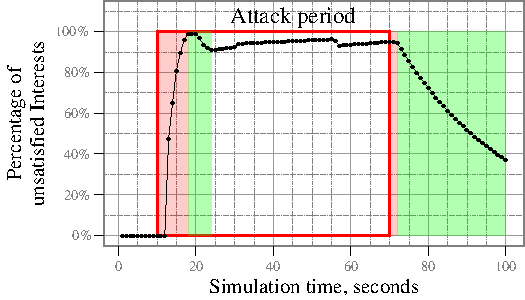
\includegraphics[scale=1]{limits}
  \caption{Dynamics of the unsatisfied Interests statistics on gateway's interface towards the attacker}
  \label{fig:ratio example}
\end{figure}


%%% Local Variables: 
%%% mode: latex
%%% TeX-master: "../paper"
%%% End: 





\end{document}
